\documentclass[12pt]{article}

% in the following lines, you may choose the packages you wish to load
\def\usepgf{true} 
\def\useminitoc{false}
\def\useglossary{false}
\def\uselineno{false}
\def\usenomencl{false} 

\usepackage[table,xcdraw, dvipsnames]{xcolor}

\usepackage{tikz}
\usetikzlibrary{shapes.geometric}

\usepackage{pgfplots} 
\pgfplotsset{width=10cm,compat=1.9} 
% \usepgfplotslibrary{external} % pour exporter séparément les figures et les importer après dans le doc. Compilation plus rapide
% \tikzexternalize[prefix=tikz/]
\synctex=1 
\usetikzlibrary{calc}
\usetikzlibrary{patterns}
\usepackage[labelformat=simple]{subcaption}
\renewcommand\thesubfigure{(\alph{subfigure})}


\usepgfplotslibrary{colorbrewer}
\usetikzlibrary{pgfplots.statistics, pgfplots.colorbrewer} % provides \pgfplotstabletranspose
\usepackage{colortbl}

% \def\firstcolor{Lavender}
% \def\secondcolor{YellowGreen}
% \def\thirdcolor{Dandelion}
% \def\fourthcolor{Goldenrod}
% \def\fifthcolor{lightgray}
% \def\sixthcolor{lightgray}
% \def\seventhcolor{lightgray}


\def\firstcolor{OrangeRed}
\def\secondcolor{YellowGreen}
\def\thirdcolor{Aquamarine}
\def\fourthcolor{Orchid}
\def\fifthcolor{Dandelion}
\def\sixthcolor{Cyan}
\def\seventhcolor{OliveGreen}

% \definecolor{firstcolor}{RGB}{255, 182, 193} % Light Pink
% \definecolor{secondcolor}{RGB}{176, 224, 230} % Powder Blue
% \definecolor{thirdcolor}{RGB}{240, 230, 140} % Light Khaki
% \definecolor{fourthcolor}{RGB}{152, 251, 152} % Pale Green
% \definecolor{fifthcolor}{RGB}{221, 160, 221} % Plum
% \definecolor{sixthcolor}{RGB}{250, 235, 215} % Antique White
% \definecolor{seventhcolor}{RGB}{245, 222, 179} % Wheat
% \definecolor{eighthcolor}{RGB}{175, 238, 238} % Pale Turquoise
% \definecolor{ninthcolor}{RGB}{255, 239, 213} % Papaya Whip
% \definecolor{tenthcolor}{RGB}{224, 255, 255} % Light Cyan

\def\myGreen{GreenYellow}
\def\myRed{Tan}
\def\backgroundcolor{gray!10}







\author{Silou}
\date{\today}
\title{Hydrofoil study}





\begin{document}  

    % \pagenumbering{roman}
    \maketitle
    

    \clearpage
    \section{Setup}
    % The geometry comes from Grabcad https://grabcad.com/library/wingsurf-hydrofoil-1 
% The following changes have been applied so that it has a span around 1 m and is aligned with $+x$:

% \begin{itemize}
%     \item \verb|surfaceTransformPoints -scale 0.03 |
%     \item \verb|surfaceTransformPoints -rotate '((1 0 0) (0 1 0))'|
%     \item \verb|surfaceTransformPoints -translate '(0 0 0.5)'|
% \end{itemize}

% In order to determine the dynamicMeshDict stuff, \verb|surfaceInertia -density 800 -referencePoint '(0 0 1)' ....stl|

\subsection{Geometry}

    The 6.50 geometry comes from onshape, export into STL in meters 
    The following changes have been applied:

    \begin{itemize}
        % \item \verb|surfaceTransformPoints -scale 0.03 |
        \item \verb|surfaceTransformPoints -translate '(0 0 0.6)'|
        \item \verb|surfaceTransformPoints -rotate '((0 0 1) (0 -0.3090169943749474 0.9510565162951535))'|
    \end{itemize}

    In order to determine the dynamicMeshDict stuff, \verb|surfaceInertia -density 100 -referencePoint '(0 0 1)' ....stl|


    Attention, faut refaire le surfaceInertia à chaque changement de roll angle 

\subsection{Mesh}
    \begin{itemize}
        \item SHM
        \item refbox around the water interface 
        \item refbox in the neigborhood of the boat (distance) 
    \end{itemize}

    \begin{table}[ht!]
        \centering\begin{tabular}{c|p{4cm}|c|c}
            Mesh & definition & \#cells & cost 15 ftt (foils - no foils)\\
            \hline
            \hline
            M0 (100k) & foils 5 6 7 \newline coque 3 4 \newline water 3 4 \newline quille 6 6 & 1.5e5 & $\approx$ 5h - ??\\
            M1 (200k)& foils 6 7 8 \newline coque 3 4 \newline water 3 4 \newline quille 6 6 & 2e5 & $\approx$ 14h - 2h \\
            M2 (300k)& foils 7 8 8 \newline coque 4 5 \newline water 3 4 \newline quille 7 7 & 3e5 & $\approx$ 18h - \\
        \end{tabular}
        \caption{Mesh sizes and cost.}
        \label{tab:meshes}
    \end{table}

    % \begin{table}[ht!]
    %     \centering\begin{tabular}{c|p{4cm}|c|c}
    %         Mesh & definition & \#cells & cost 10 ftt\\
    %         \hline
    %         \hline
    %         M0 & foils 6 6 \newline coque 3 4 \newline water 3 3 \newline quille 5 5 & 1.1e5 & \textasciitilde \\
    %         M1 & foils 7 7 \newline coque 4 5 \newline water 3 4 \newline quille 6 6 & 2.1e5 & \textasciitilde 60 min\\
    %         M2 & foils 7 7 \newline coque 5 6 \newline water 3 4 \newline quille 6 6 & 1e7 & \textasciitilde 90 min\\
    %     \end{tabular}
    %     \caption{Mesh sizes and cost.}
    %     \label{tab:meshes}
    % \end{table}




% \subsection{Numerical parameters}

%     \begin{itemize}
%         \item interFoam, multiphase 
%         \item pimple loop 
%         \item second order schemes 
%         \item "pseudo steady state" 6DOF : large relaxation and damping, but necessarily transient 
%     \end{itemize}

% \subsection{Postprocessing}
%     \begin{itemize}
%         \item Surfaces 
%         \item Forces 
%         \item DES LOGS DE 6DOF À METTRE EN PLACE  
%     \end{itemize}


    
% surfaceTransformPoints -rotate '((0 1 0) (1 0 0))' coque.stl coque_x.stl
% surfaceTransformPoints -rotate '((0 1 0) (1 0 0))' foils.stl foils_x.stl
% surfaceTransformPoints -rotate '((0 1 0) (1 0 0))' quille.stl quille_x.stl

% surfaceTransformPoints -rotate '((0 0 1) (0 -0.25881904510252074 0.9659258262890683))' coque_x.stl coque_x_gite.stl
% surfaceTransformPoints -rotate '((0 0 1) (0 -0.25881904510252074 0.9659258262890683))' foils_x.stl foils_x_gite.stl
% surfaceTransformPoints -rotate '((0 0 1) (0 -0.25881904510252074 0.9659258262890683))' quille_x.stl quille_x_gite.stl


% surfaceTransformPoints -rotate '((0 1 0) (1 0 0))' foils4.stl foils_x.stl
% surfaceTransformPoints -rotate '((0 1 0) (1 0 0))' refBox_LE.stl refBox_LE_x.stl
% surfaceTransformPoints -rotate '((0 1 0) (1 0 0))' refBox_TE.stl refBox_TE_x.stl

% surfaceTransformPoints -rotate '((0 0 1) (0 -0.25881904510252074 0.9659258262890683))' foils_x.stl foils_x_gite.stl
% surfaceTransformPoints -rotate '((0 0 1) (0 -0.25881904510252074 0.9659258262890683))' refBox_LE_x.stl refBox_LE_x_gite.stl
% surfaceTransformPoints -rotate '((0 0 1) (0 -0.25881904510252074 0.9659258262890683))' refBox_TE_x.stl refBox_TE_x_gite.stl


    \clearpage
    \section{Results}
    % \subsection{Stuff}

% Fig. \ref{fig:lift_drag} shows the lift and drag time evolution, and Fig. \ref{fig:lift_drag_u} the lift and drag steady states converged  as functions of velocity.


% \begin{figure}[ht!]
%     \centering
%     \begin{subfigure}{0.48\textwidth}
%         \begin{tikzpicture}
%             \begin{axis}[
%                 xmin=0, xmax=6,
%                 ymin=0.3e5, ymax=0.8e5,
%                 legend pos=north east,
%                 xlabel = {t (s)},
%                 ylabel = {Lift (N)},
%                 no markers,
%                 every axis plot/.append style={ultra thick},
%                 width=0.98\textwidth, 
%                 ]
%                 \addplot +[mark=none, color=\firstcolor, style=solid] table[y expr=\thisrowno{3}] {curves/fixed/force_3.dat};
%                 \addplot +[mark=none, color=\secondcolor, style=solid] table[y expr=\thisrowno{3}] {curves/fixed/force_5.dat};
%                 \addplot +[mark=none, color=\thirdcolor, style=solid] table[y expr=\thisrowno{3}] {curves/fixed/force_7.dat};
%                 \addplot +[mark=none, color=\fourthcolor, style=solid] table[y expr=\thisrowno{3}] {curves/fixed/force_9.dat};
%                 \addplot +[mark=none, color=\fifthcolor, style=solid] table[y expr=\thisrowno{3}] {curves/fixed/force_11.dat};
%                 \addplot +[mark=none, color=\sixthcolor, style=solid] table[y expr=\thisrowno{3}] {curves/fixed/force_13.dat};
%                 \addplot +[mark=none, color=\seventhcolor, style=solid] table[y expr=\thisrowno{3}] {curves/fixed/force_15.dat};
%             \end{axis} 
%         \end{tikzpicture}   
%         \caption{Lift evolution.}
%         \label{fig:lift}
%     \end{subfigure}
%     \begin{subfigure}{0.48\textwidth}
%         \begin{tikzpicture}
%             \begin{axis}[
%                 xmin=0, xmax=6,
%                 ymin=0, ymax=2e4,
%                 legend pos=north east,
%                 xlabel = {t (s)},
%                 ylabel = {Drag (N)},
%                 no markers,
%                 every axis plot/.append style={ultra thick},
%                 width=0.98\textwidth, 
%                 ]
%                 \addplot +[mark=none, color=\firstcolor, style=solid] table[y expr=-\thisrowno{1}] {curves/fixed/force_3.dat};
%                 \addplot +[mark=none, color=\secondcolor, style=solid] table[y expr=-\thisrowno{1}] {curves/fixed/force_5.dat};
%                 \addplot +[mark=none, color=\thirdcolor, style=solid] table[y expr=-\thisrowno{1}] {curves/fixed/force_7.dat};
%                 \addplot +[mark=none, color=\fourthcolor, style=solid] table[y expr=-\thisrowno{1}] {curves/fixed/force_9.dat};
%                 \addplot +[mark=none, color=\fifthcolor, style=solid] table[y expr=-\thisrowno{1}] {curves/fixed/force_11.dat};
%                 \addplot +[mark=none, color=\sixthcolor, style=solid] table[y expr=-\thisrowno{1}] {curves/fixed/force_13.dat};
%                 \addplot +[mark=none, color=\seventhcolor, style=solid] table[y expr=-\thisrowno{1}] {curves/fixed/force_15.dat};
%             \end{axis}
%         \end{tikzpicture}   
%         \caption{Drag evolution.}
%         \label{fig:drag}
%     \end{subfigure}

%     \begin{tikzpicture}
%         \begin{axis}[
%             hide axis,
%             xmin=0, xmax=1, ymin=0, ymax=1,
%             legend columns=3, % -1 pour aligner horizontalement, 1 pour aligner verticalement
%             legend entries={$u=3$, $u=5$, $u=7$, $u=9$, $u=11$, $u=13$, $u=15$},
%             % cycle list/Set2-8,
%             width=0.25\textwidth
%         ]
%         \addlegendimage{ultra thick, \firstcolor}
%         \addlegendimage{ultra thick, \secondcolor}
%         \addlegendimage{ultra thick, \thirdcolor}
%         \addlegendimage{ultra thick, \fourthcolor}
%         \addlegendimage{ultra thick, \fifthcolor}
%         \addlegendimage{ultra thick, \sixthcolor}
%         \addlegendimage{ultra thick, \seventhcolor}
%         \end{axis}
%     \end{tikzpicture}
%     \caption{Lift and drag evolution - fixed boat.}
%     \label{fig:lift_drag}
% \end{figure}



% \begin{figure}[ht!]
%     \centering
%     \begin{subfigure}{0.48\textwidth}
%         \begin{tikzpicture}
%             \begin{axis}[
%                 xmin=0, xmax=15,
%                 ymin=0.3e5, ymax=0.8e5,
%                 legend pos=north east,
%                 xlabel = {u (m/s)},
%                 ylabel = {Lift (N)},
%                 every axis plot/.append style={ultra thick},
%                 width=0.98\textwidth, 
%                 ]
%                 \addplot +[mark=*, mark options={fill=\firstcolor}, color=\firstcolor, style=solid] table[y expr=\thisrowno{1}] {curves/fixed/force_speed};
%                 \addplot +[mark=*, mark options={fill=\firstcolor}, color=\firstcolor, style=dotted] table[y expr=\thisrowno{1}] {curves/fixed/force_nofoil_speed};
%             \end{axis} 
%         \end{tikzpicture}   
%         \caption{Lift evolution.}
%         \label{fig:lift_u}
%     \end{subfigure}
%     \begin{subfigure}{0.48\textwidth}
%         \begin{tikzpicture}
%             \begin{axis}[
%                 xmin=0, xmax=15,
%                 ymin=0, ymax=3e4,
%                 legend pos=north east,
%                 xlabel = {u (m/s)},
%                 ylabel = {Drag (N)},
%                 every axis plot/.append style={ultra thick},
%                 width=0.98\textwidth, 
%                 ]
%                 \addplot +[mark=*, mark options={fill=\firstcolor}, color=\firstcolor, style=solid] table[y expr=\thisrowno{2}] {curves/fixed/force_speed};
%                 \addplot +[mark=*, mark options={fill=\firstcolor}, color=\firstcolor, style=dotted] table[y expr=\thisrowno{2}] {curves/fixed/force_nofoil_speed};
%             \end{axis}
%         \end{tikzpicture}   
%         \caption{Drag evolution.}
%         \label{fig:drag_u}
%     \end{subfigure}
%     \begin{tikzpicture}
%         \begin{axis}[
%             hide axis,
%             xmin=0, xmax=1, ymin=0, ymax=1,
%             legend columns=3, % -1 pour aligner horizontalement, 1 pour aligner verticalement
%             legend entries={hull and foil, hull only},
%             % cycle list/Set2-8,
%             width=0.25\textwidth
%         ]
%         \addlegendimage{ultra thick, mark=*, mark options={fill=\firstcolor}, solid, \firstcolor}
%         \addlegendimage{ultra thick, mark=*, mark options={fill=\firstcolor}, dotted, \firstcolor}
%         \end{axis}
%     \end{tikzpicture}
%     \caption{Lift and drag evolution - fixed boat.}
%     \label{fig:lift_drag_u}
% \end{figure}


\subsection{Force time evolution and mesh convergence}

    \begin{figure}[ht!]
        \centering
        \begin{subfigure}{0.48\textwidth}
            \begin{tikzpicture}
                \begin{axis}[
                    xlabel={time (s)},
                    ylabel={Lift (N)},
                    % xmin=0, xmax=1e4, 
                    % ymin=1.3e4, ymax=1.5e4,
                    ymajorgrids=true,xmajorgrids=true,
                    legend pos=south east,
                    width=0.98\textwidth,
                    axis background/.style={fill=\backgroundcolor}
                    ]
                    \addplot +[mark=None, style=ultra thick, color=\firstcolor, style=ultra thick, style=solid] table[x expr=(\thisrowno{0}), y expr=(\thisrowno{3})] {curves/forces/force_200k};
                    \addplot +[mark=None, style=ultra thick, color=\secondcolor, style=ultra thick, style=solid] table[x expr=(\thisrowno{0}), y expr=(\thisrowno{3})] {curves/forces/force_300k};
                    \addplot +[mark=None, style=ultra thick, color=\thirdcolor, style=ultra thick, style=solid] table[x expr=(\thisrowno{0}), y expr=(\thisrowno{3})] {curves/forces/force_200k_nofoils};
                \end{axis}
            \end{tikzpicture}
            \caption{Lift evolution.}
            \label{fig:lift_evolution}
        \end{subfigure}
        \begin{subfigure}{0.48\textwidth}
            \begin{tikzpicture}
                \begin{axis}[
                    xlabel={time (s)},
                    ylabel={Drag (N)},
                    % xmin=0, xmax=20000,
                    % ymin=3.7e3, ymax=4.5e3,
                    ymajorgrids=true,xmajorgrids=true,
                    legend pos=south east,
                    width=0.98\textwidth,
                    axis background/.style={fill=\backgroundcolor}
                    ]
                    \addplot +[mark=None, style=ultra thick, color=\firstcolor, style=ultra thick, style=solid] table[x expr=(\thisrowno{0}), y expr=(-\thisrowno{1})] {curves/forces/force_200k};
                    \addplot +[mark=None, style=ultra thick, color=\secondcolor, style=ultra thick, style=solid] table[x expr=(\thisrowno{0}), y expr=(-\thisrowno{1})] {curves/forces/force_300k};
                    \addplot +[mark=None, style=ultra thick, color=\thirdcolor, style=ultra thick, style=solid] table[x expr=(\thisrowno{0}), y expr=(-\thisrowno{1})] {curves/forces/force_200k_nofoils};
                \end{axis}
            \end{tikzpicture}
            \caption{Drag evolution.}
            \label{fig:drag_evolution}
        \end{subfigure}
        \begin{subfigure}{0.48\textwidth}
            \begin{tikzpicture}
                \begin{axis}[
                    xlabel={time (s)},
                    ylabel={z (m)},
                    % xmin=0, xmax=20000,
                    % ymin=3.7e3, ymax=4.5e3,
                    ymajorgrids=true,xmajorgrids=true,
                    legend pos=south east,
                    width=0.98\textwidth,
                    axis background/.style={fill=\backgroundcolor}
                    ]
                    \addplot +[mark=None, style=ultra thick, color=\firstcolor, style=ultra thick, style=solid] table[x expr=(\thisrowno{0}), y expr=(\thisrowno{3})] {curves/rigidBodyMotionDisplacement/tq_200k};
                    \addplot +[mark=None, style=ultra thick, color=\secondcolor, style=ultra thick, style=solid] table[x expr=(\thisrowno{0}), y expr=(\thisrowno{3})] {curves/rigidBodyMotionDisplacement/tq_300k};
                    \addplot +[mark=None, style=ultra thick, color=\thirdcolor, style=ultra thick, style=solid] table[x expr=(\thisrowno{0}), y expr=(\thisrowno{3})] {curves/rigidBodyMotionDisplacement/tq_200k_nofoils};
                \end{axis}
            \end{tikzpicture}
            \caption{Vertical displacement evolution.}
            \label{fig:drag_evolution}
        \end{subfigure}
        
        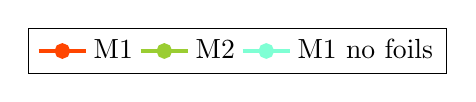
\begin{tikzpicture}
            \begin{axis}[
                hide axis,
                xmin=0, xmax=1, ymin=0, ymax=1,
                legend columns=-1, % -1 pour aligner horizontalement, 1 pour aligner verticalement
                legend entries={M1, M2, M1 no foils},
                width=0.25\textwidth
                ]
                \addlegendimage{ultra thick, mark=*, \firstcolor}
                \addlegendimage{ultra thick, mark=*, \secondcolor}
                \addlegendimage{ultra thick, mark=*, \thirdcolor}
            \end{axis}
        \end{tikzpicture}

        \caption{Convergence of the metrics with the iterations.}
        \label{fig:meshConvergence}
    \end{figure}

    

    % \begin{figure}[ht!]
    %     \centering
    %     \begin{subfigure}{0.3\textwidth}
    %         \begin{tikzpicture}
    %             \begin{axis}[
    %                 % xlabel={mesh},
    %                 % ylabel={Lift},
    %                 % xmin=0, xmax=1e4, 
    %                 % ymin=1.3e4, ymax=1.5e4,
    %                 ymajorgrids=true,xmajorgrids=true,
    %                 legend pos=south east,
    %                 width=0.98\textwidth,
    %                 % title={z},
    %                 width=0.98\textwidth,
    %                 axis background/.style={fill=\backgroundcolor}
    %                 ]
    %                 \addplot +[mark=None, style=ultra thick, color=\firstcolor, style=ultra thick, style=solid] table[x expr=(\thisrowno{0}), y expr=(\thisrowno{1})] {curves/convergence/meshConvergence};
    %             \end{axis}
    %         \end{tikzpicture}
    %         \caption{Displacement (m).}
    %         \label{fig:lift_evolution}
    %     \end{subfigure}
    %     \begin{subfigure}{0.3\textwidth}
    %         \begin{tikzpicture}
    %             \begin{axis}[
    %                 % xlabel={time},
    %                 % ylabel={Drag},
    %                 % xmin=0, xmax=20000,
    %                 % title={Lift},
    %                 width=0.98\textwidth,
    %                 % ymin=3.7e3, ymax=4.5e3,
    %                 ymajorgrids=true,xmajorgrids=true,
    %                 legend pos=south east,
    %                 width=0.98\textwidth,
    %                 axis background/.style={fill=\backgroundcolor}
    %                 ]
    %                 \addplot +[mark=None, style=ultra thick, color=\firstcolor, style=ultra thick, style=solid] table[x expr=(\thisrowno{0}), y expr=(\thisrowno{2})] {curves/convergence/meshConvergence};
    %             \end{axis}
    %         \end{tikzpicture}
    %         \caption{Lift (N).}
    %         \label{fig:drag_evolution}
    %     \end{subfigure}
    %     \begin{subfigure}{0.3\textwidth}
    %         \begin{tikzpicture}
    %             \begin{axis}[
    %                 % xlabel={time},
    %                 % ylabel={elevation},
    %                 % xmin=0, xmax=20000,
    %                 % title={Drag},
    %                 width=0.98\textwidth,
    %                 % ymin=3.7e3, ymax=4.5e3,
    %                 ymajorgrids=true,xmajorgrids=true,
    %                 legend pos=south east,
    %                 width=0.98\textwidth,
    %                 axis background/.style={fill=\backgroundcolor}
    %                 ]
    %                 \addplot +[mark=None, style=ultra thick, color=\firstcolor, style=ultra thick, style=solid] table[x expr=(\thisrowno{0}), y expr=(\thisrowno{3})] {curves/convergence/meshConvergence};
    %             \end{axis}
    %         \end{tikzpicture}
    %         \caption{Drag (N).}
    %         \label{fig:drag_evolution}
    %     \end{subfigure}
    %     \caption{.}
    %     \label{fig:meshConvergence}
    % \end{figure}



    \cleardoublepage
    \section{Phase 1: computation of the boat velocity}
    %!TEX root = ../main.tex
\subsection{Concept}
    \label{section:iterative_process}
    The unknown of the problem, the boat velocity $\mathbf{u}_b$, is considered in the computation as a boundary condition. In order to determine its value, an iterative process is proposed. 
    The rolling/pitch movement is neglected for now, a "gite" of 15° is considered and only the vertical displacement is allowed in the rigid body motion. 


    \begin{enumerate}
        \item The computation is started with a velocity chosen at random, $U_0 = 3$m/s for instance. 
        \item The drag $\mathbf{D}$ due to water is computed as a postprocessing step after a fully converged M0M1 computation and an average over around 10 flow through times is taken. 
        \item The speed triangle is set to determine the apparent wind, see Fig. \ref{fig:speedtriangle}
        \item The estimation of the thrust applied by the wind $\mathbf{T}$ is detailed in section \ref{section:wind_force}.
        \item The numerically computed drag $\mathbf{D}$ is compared to the estimated thrust $\mathbf{T}$, $\alpha=\frac{||\mathbf{T}||}{||\mathbf{D}||}$.
        \item If $\frac{\alpha_n-\alpha_{n-1}}{\alpha_{n-1}} > 0.01$, the BC is updated $\mathbf{u}_b^{n+1}=\mathbf{u}_b^{n}*\frac{\mathbf{T}}{\mathbf{D}}$ and another computation is launched. 
        \item To prevent overestimation and oscillatory behaviours, a blending factor $r_n$ is used, $\mathbf{u}_b^{n+1}=\mathbf{u}_b^{n}*(1+\alpha r_n(\alpha-1))$. Choosing a low $r_n$ at the beginning and increasing it with $n$ is a good way of proceeding. 
    \end{enumerate}


\subsection{Wind force}
    \label{section:wind_force}
    Two different modes are possible: upwind or downwind. In the former, the sails works as an airfoil with an attached flow, the lift and drag are computed. In the latter, it acts as a planar plate and only the drag of this surface is taken into account (approximated as the product of the sail surface by the stagnation pressure).
    
    In the upwind configuration, lift and drag are computed as follows, with $u$ the scalar product between the apparent wind and a unit vector \textbf{aligned} with the sail:
    \begin{eqnarray}
        F_l = \frac{1}{2}\rho u^2 S C_l, \\ 
        F_d = \frac{1}{2}\rho u^2 S C_d.
        \label{eqn:windforce_upwind}
    \end{eqnarray}

    In the downwind configuration, lift and drag are computed as follows, with $p_s=\frac{1}{2}\rho u^2$, $\alpha=0.5$ a bullshit factor, and $u$ the scalar product between the apparent wind and a unit vector \textbf{perpendicular} to the sail:
    \begin{eqnarray}
        F_l = 0, \\ 
        F_d = \alpha \ S \ p_s.
        \label{eqn:windforce_downwind}
    \end{eqnarray}

    These are expressed in the sail reference frame. The thrust $T$, is the projection of this force on the $x$ axis. 

    In order to determine wether the boat is in upwind or downwind mode (this may change in the iterative algorithm), both modes are computed and the highest thrust value is kept.  

    \begin{figure}[ht!]
        \centering
        \begin{minipage}{0.65\textwidth}
            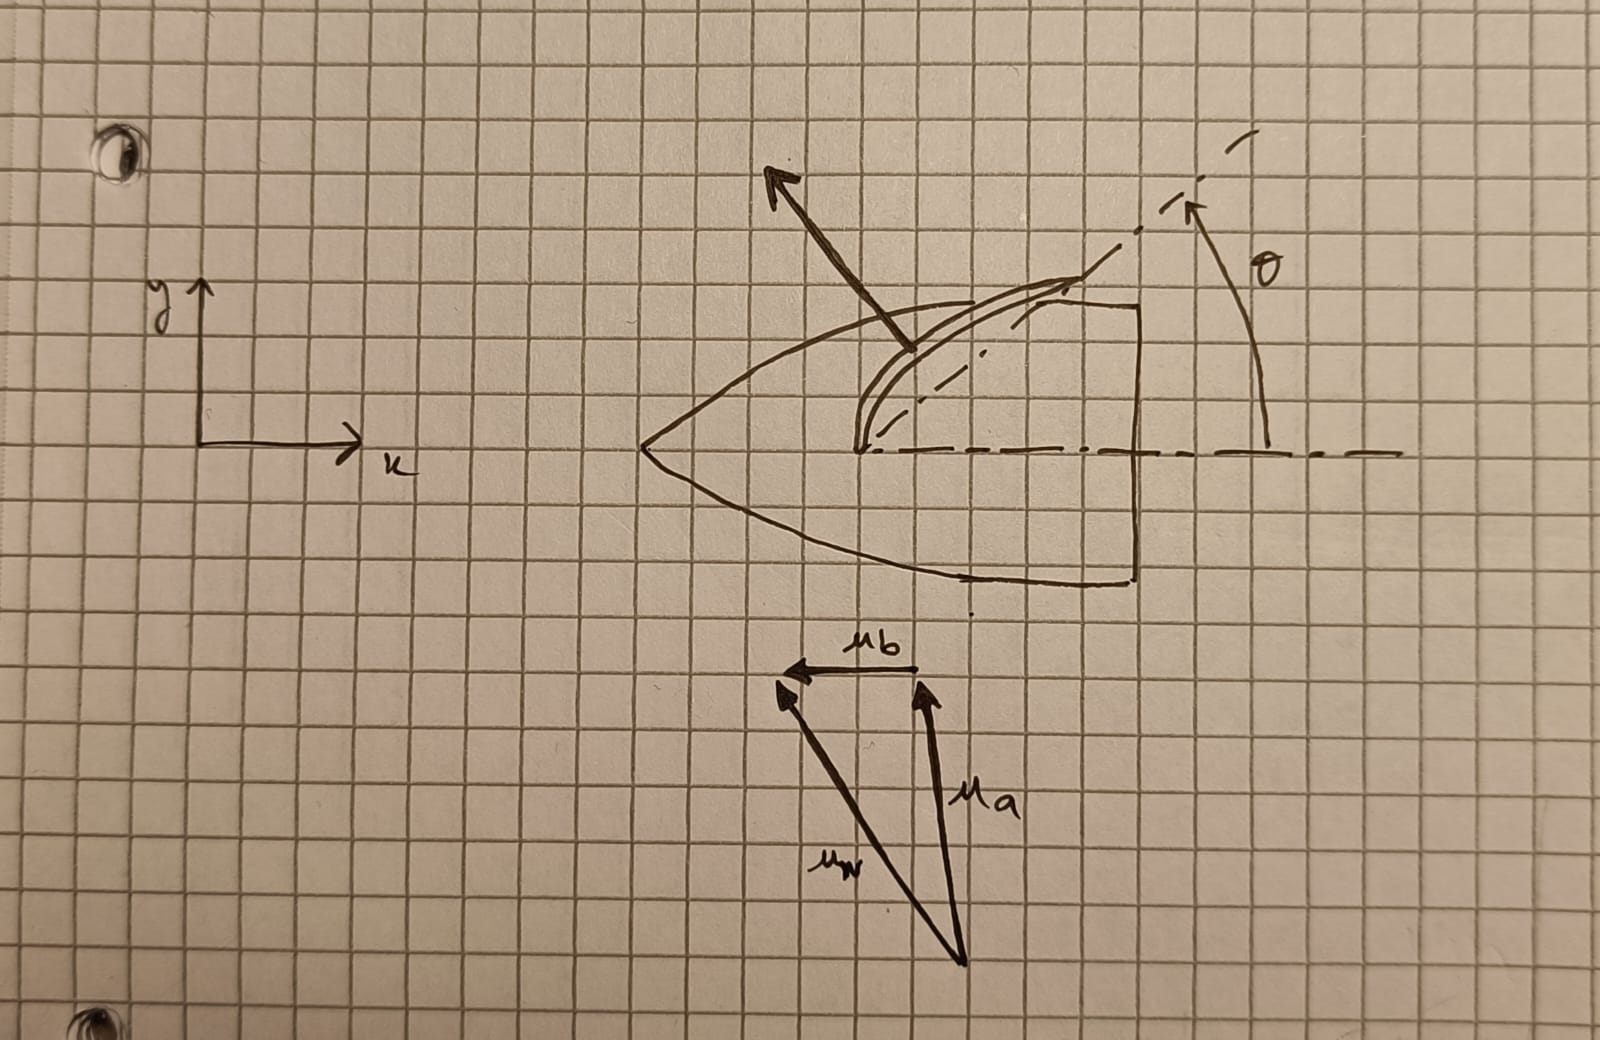
\includegraphics[width=0.99\textwidth]{figures/axes.jpeg}% \\
        \end{minipage}
        \begin{minipage}{0.34\textwidth}
            \vfill
            \begin{tabular}{c|c}
                $\mathbf{u}_w$ & wind speed \\
                $\mathbf{u}_b$ & boat speed \\
                $\mathbf{u}_a$ & apparent wind
            \end{tabular}
            \vfill
        \end{minipage}
        % $U_w$ : wind speed \\
        % $U$ : boat speed \\
        % $U_a$ : apparent wind
        
        \caption{Notations}
        \label{fig:speedtriangle}
    \end{figure}

\subsection{Initial velocity }
    In order to accelerate the computation. The initial velocity BC $\mathbf{u}_b^0$ may be guessed with the same iterative algorithm as in \ref{section:iterative_process}. The only difference lies in the determination of the drag: instead of an accurate but costly CFD computed drag, we estimate it with 
    \begin{eqnarray}
        D'+D'' = \frac{1}{2}\rho u^2 \left(S' C_d' +S'' C_d''\right), \\ 
        \label{eqn:drag_estimation}
    \end{eqnarray}
    with $S'= 0.9$ the projected wet surface in an x-aligned plane, and $S''= 8.64 $ the wet surface. This decomposition allows us to take into account both the drag due to pressure distribution, and the one due to friction. 

    The determination of $C_d'$ and $C_d''$ is made numerically with OpenFOAM results. 

    \begin{table}[ht!]
        \centering
        \begin{tabular}{p{4cm}|c|c|c|c|c}
            Run & Velocity & $D'=$ & $D''$ & $C_d'=2*/\rho u^2 S'$ & $C_d''=2*/\rho u^2 S'$ \\
            \hline  
            underdamped 150 & 6.8 & 1700 & 600 & 0.08941 & 0.00328 \\
            critical 100 & 10 & 2700 & 900 & 0.142 & 0.00493 \\
            best upwind & 5.037 & 1327 & 403 & 0.116 & 0.003676 \\  
            100 deg & 5.12 & 1460 & 375 & 0.1238 & 0.003311 \\
        \end{tabular}
        \caption{Numerical estimation of the drag coefficients on the hull}
        \label{tab:dragCoeffHull}
    \end{table}


\clearpage
\subsection{Results}
    Fig. \ref{fig:iterative_process} shows the convergence of the inlet velocity BC $\mathbf{u_b}$ with an initial condition $\mathbf{u_b}^0 = 5$ m/s and a wind $\mathbf{u_w} = \langle 1.73, 9.85\rangle$ m/s (15 knots, 80 deg), without foils or keel, on mesh M1 (M0 and M1 without foils are the same). The relaxation factor $r_n$ varies linearly from 0.2 to 0.8. The process converged in 3h (4 iterations). 

    \begin{figure}[ht!]
        \centering
        \begin{subfigure}{0.49\textwidth}
            \begin{tikzpicture}
                \begin{axis}[
                    xlabel={Iteration},
                    ylabel={$\mathbf{u}_b$ (m/s)},
                    % xmin=0, xmax=10,
                    % ymin=0, ymax=6,
                    ymajorgrids=true,xmajorgrids=true,
                    legend pos=south east,
                    width=0.98\textwidth,
                    axis background/.style={fill=\backgroundcolor}
                    ]
                    \addplot +[mark=None, style=ultra thick, color=\firstcolor, style=ultra thick, style=solid] table[x expr=(\thisrowno{0}), y expr=(\thisrowno{1})] {curves/iterativeProcess/iterative_process_result_u1.7_9.8};
                \end{axis}
            \end{tikzpicture}
            \caption{Velocity}
        \end{subfigure}
        \begin{subfigure}{0.49\textwidth}
            \begin{tikzpicture}
                \begin{axis}[
                    xlabel={Iteration},
                    ylabel={Forces (N)},
                    % xmin=0, xmax=10,
                    % ymin=0, ymax=6,
                    ymajorgrids=true,xmajorgrids=true,
                    legend pos=south east,
                    width=0.98\textwidth,
                    axis background/.style={fill=\backgroundcolor}
                    ]
                    \addplot +[mark=None, style=ultra thick, color=\firstcolor, style=ultra thick, style=solid] table[x expr=(\thisrowno{0}), y expr=(\thisrowno{2})] {curves/iterativeProcess/iterative_process_result_u1.7_9.8};
                    \addplot +[mark=None, style=ultra thick, color=\secondcolor, style=ultra thick, style=solid] table[x expr=(\thisrowno{0}), y expr=(-\thisrowno{3})] {curves/iterativeProcess/iterative_process_result_u1.7_9.8};
                    \legend{$T$, $-D$}
                \end{axis}
            \end{tikzpicture}
            \caption{Forces}
        \end{subfigure}
            
        \caption{Iterative determination of the velocity inlet BC for a wind speed of $\langle -10, 0\rangle$ m/s (15 knots, pure downwind).}
        \label{fig:iterative_process}
    \end{figure}

    The forces for the last iteration are the following : 
    \begin{figure}[ht!]
        \centering
        \begin{subfigure}{0.32\textwidth}
            \begin{tikzpicture}
                \begin{axis}[
                    xlabel={time (s)},
                    % ylabel={Lift (N)},
                    ymajorgrids=true,xmajorgrids=true,
                    legend pos=south east,
                    width=0.98\textwidth,
                    axis background/.style={fill=\backgroundcolor}
                    ]
                    \addplot +[mark=None, style=ultra thick, color=\firstcolor, style=ultra thick, style=solid] table[x expr=(\thisrowno{0}), y expr=(\thisrowno{3})] {curves/iterativeProcess/forces_u1.7_9.8};
                \end{axis}
            \end{tikzpicture}
            \caption{$L$ (N)}
            \label{fig:lift_evolution}
        \end{subfigure}
        \begin{subfigure}{0.32\textwidth}
            \begin{tikzpicture}
                \begin{axis}[
                    xlabel={time (s)},
                    % ylabel={Drag (N)},
                    ymajorgrids=true,xmajorgrids=true,
                    legend pos=south east,
                    width=0.98\textwidth,
                    axis background/.style={fill=\backgroundcolor}
                    ]
                    \addplot +[mark=None, style=ultra thick, color=\firstcolor, style=ultra thick, style=solid] table[x expr=(\thisrowno{0}), y expr=(-\thisrowno{1})] {curves/iterativeProcess/forces_u1.7_9.8};
                \end{axis}
            \end{tikzpicture}
            \caption{$D$ (N)}
            \label{fig:drag_evolution}
        \end{subfigure}
        \begin{subfigure}{0.32\textwidth}
            \begin{tikzpicture}
                \begin{axis}[
                    xlabel={time (s)},
                    % ylabel={z (m)},
                    ymajorgrids=true,xmajorgrids=true,
                    legend pos=south east,
                    width=0.98\textwidth,
                    axis background/.style={fill=\backgroundcolor}
                    ]
                    \addplot +[mark=None, style=ultra thick, color=\firstcolor, style=ultra thick, style=solid] table[x expr=(\thisrowno{0}), y expr=(\thisrowno{3})] {curves/iterativeProcess/tq_u1.7_9.8};
                \end{axis}
            \end{tikzpicture}
            \caption{$z$ (m)}
            \label{fig:drag_evolution}
        \end{subfigure}
        \caption{Last computation of the iterative process, evolution of forces and vertical displacement.}
        \label{fig:meshConvergence}
    \end{figure}


    \clearpage
    Same thing in Fig. \ref{fig:iterative_process_2}, with an initial condition $\mathbf{u_b}^0 = 7$ m/s and a wind $\mathbf{u_w} = \langle -1.73, 9.85\rangle$ m/s (15 knots, 100 deg), without foils or keel, on mesh M1 (M0 and M1 without foils are the same). The relaxation factor $r_n$ varies linearly from 0.2 to 0.8. The process converged in 2h (3 iterations). 

    \begin{figure}[ht!]
        \centering
        \begin{subfigure}{0.49\textwidth}
            \begin{tikzpicture}
                \begin{axis}[
                    xlabel={Iteration},
                    ylabel={$\mathbf{u}_b$ (m/s)},
                    ymajorgrids=true,xmajorgrids=true,
                    legend pos=south east,
                    width=0.98\textwidth,
                    axis background/.style={fill=\backgroundcolor}
                    ]
                    \addplot +[mark=None, style=ultra thick, color=\firstcolor, style=ultra thick, style=solid] table[x expr=(\thisrowno{0}), y expr=(\thisrowno{1})] {curves/iterativeProcess/iterative_process_result_um1.7_9.8};
                \end{axis}
            \end{tikzpicture}
            \caption{Velocity}
        \end{subfigure}
        \begin{subfigure}{0.49\textwidth}
            \begin{tikzpicture}
                \begin{axis}[
                    xlabel={Iteration},
                    ylabel={Forces (N)},
                    ymajorgrids=true,xmajorgrids=true,
                    legend pos=south east,
                    width=0.98\textwidth,
                    axis background/.style={fill=\backgroundcolor}
                    ]
                    \addplot +[mark=None, style=ultra thick, color=\firstcolor, style=ultra thick, style=solid] table[x expr=(\thisrowno{0}), y expr=(\thisrowno{2})] {curves/iterativeProcess/iterative_process_result_um1.7_9.8};
                    \addplot +[mark=None, style=ultra thick, color=\secondcolor, style=ultra thick, style=solid] table[x expr=(\thisrowno{0}), y expr=(-\thisrowno{3})] {curves/iterativeProcess/iterative_process_result_um1.7_9.8};
                    \legend{$T$, $-D$}
                \end{axis}
            \end{tikzpicture}
            \caption{Forces}
        \end{subfigure}
            
        \caption{Iterative determination of the velocity inlet BC for a wind speed of $\langle -10, 0\rangle$ m/s (15 knots, pure downwind).}
        \label{fig:iterative_process_2}
    \end{figure}

    The forces for the last iteration are the following : 
    \begin{figure}[ht!]
        \centering
        \begin{subfigure}{0.32\textwidth}
            \begin{tikzpicture}
                \begin{axis}[
                    xlabel={time (s)},
                    % ylabel={Lift (N)},
                    ymajorgrids=true,xmajorgrids=true,
                    legend pos=south east,
                    width=0.98\textwidth,
                    axis background/.style={fill=\backgroundcolor}
                    ]
                    \addplot +[mark=None, style=ultra thick, color=\firstcolor, style=ultra thick, style=solid] table[x expr=(\thisrowno{0}), y expr=(\thisrowno{3})] {curves/iterativeProcess/forces_um1.7_9.8};
                \end{axis}
            \end{tikzpicture}
            \caption{$L$ (N)}
            \label{fig:lift_evolution}
        \end{subfigure}
        \begin{subfigure}{0.32\textwidth}
            \begin{tikzpicture}
                \begin{axis}[
                    xlabel={time (s)},
                    ymajorgrids=true,xmajorgrids=true,
                    legend pos=south east,
                    width=0.98\textwidth,
                    axis background/.style={fill=\backgroundcolor}
                    ]
                    \addplot +[mark=None, style=ultra thick, color=\firstcolor, style=ultra thick, style=solid] table[x expr=(\thisrowno{0}), y expr=(-\thisrowno{1})] {curves/iterativeProcess/forces_um1.7_9.8};
                \end{axis}
            \end{tikzpicture}
            \caption{$D$ (N)}
            \label{fig:drag_evolution}
        \end{subfigure}
        \begin{subfigure}{0.32\textwidth}
            \begin{tikzpicture}
                \begin{axis}[
                    xlabel={time (s)},
                    ymajorgrids=true,xmajorgrids=true,
                    legend pos=south east,
                    width=0.98\textwidth,
                    axis background/.style={fill=\backgroundcolor}
                    ]
                    \addplot +[mark=None, style=ultra thick, color=\firstcolor, style=ultra thick, style=solid] table[x expr=(\thisrowno{0}), y expr=(\thisrowno{3})] {curves/iterativeProcess/tq_um1.7_9.8};
                \end{axis}
            \end{tikzpicture}
            \caption{$z$ (m)}
            \label{fig:drag_evolution}
        \end{subfigure}
        \caption{Last computation of the iterative process, evolution of forces and vertical displacement.}
        \label{fig:meshConvergence}
    \end{figure}


\clearpage
    Same, $\mathbf{u_b}$ with an initial condition $\mathbf{u_b}^0 = 7.4$ m/s and a wind $\mathbf{u_w} = \langle 1.73, 9.85\rangle$ m/s, exporting from 30 to 35 ftt. 

    \begin{figure}[ht!]
        \centering
        \begin{subfigure}{0.49\textwidth}
            \begin{tikzpicture}
                \begin{axis}[
                    xlabel={Iteration},
                    ylabel={$\mathbf{u}_b$ (m/s)},
                    % xmin=0, xmax=10,
                    % ymin=0, ymax=6,
                    ymajorgrids=true,xmajorgrids=true,
                    legend pos=south east,
                    width=0.98\textwidth,
                    axis background/.style={fill=\backgroundcolor}
                    ]
                    \addplot +[mark=None, style=ultra thick, color=\firstcolor, style=ultra thick, style=solid] table[x expr=(\thisrowno{0}), y expr=(\thisrowno{1})] {curves/iterativeProcess/iterative_process_result_u1.7_9.8_v2};
                \end{axis}
            \end{tikzpicture}
            \caption{Velocity}
        \end{subfigure}
        \begin{subfigure}{0.49\textwidth}
            \begin{tikzpicture}
                \begin{axis}[
                    xlabel={Iteration},
                    ylabel={Forces (N)},
                    % xmin=0, xmax=10,
                    % ymin=0, ymax=6,
                    ymajorgrids=true,xmajorgrids=true,
                    legend pos=south east,
                    width=0.98\textwidth,
                    axis background/.style={fill=\backgroundcolor}
                    ]
                    \addplot +[mark=None, style=ultra thick, color=\firstcolor, style=ultra thick, style=solid] table[x expr=(\thisrowno{0}), y expr=(\thisrowno{2})] {curves/iterativeProcess/iterative_process_result_u1.7_9.8_v2};
                    \addplot +[mark=None, style=ultra thick, color=\secondcolor, style=ultra thick, style=solid] table[x expr=(\thisrowno{0}), y expr=(-\thisrowno{3})] {curves/iterativeProcess/iterative_process_result_u1.7_9.8_v2};
                    \legend{$T$, $-D$}
                \end{axis}
            \end{tikzpicture}
            \caption{Forces}
        \end{subfigure}
            
        \caption{Iterative determination of the velocity inlet BC for a wind speed of $\langle -10, 0\rangle$ m/s (15 knots, pure downwind).}
        \label{fig:iterative_process}
    \end{figure}

    The forces for the last iteration are the following : 
    \begin{figure}[ht!]
        \centering
        \begin{subfigure}{0.32\textwidth}
            \begin{tikzpicture}
                \begin{axis}[
                    xlabel={time (s)},
                    % ylabel={Lift (N)},
                    ymajorgrids=true,xmajorgrids=true,
                    legend pos=south east,
                    width=0.98\textwidth,
                    axis background/.style={fill=\backgroundcolor}
                    ]
                    \addplot +[mark=None, style=ultra thick, color=\firstcolor, style=ultra thick, style=solid] table[x expr=(\thisrowno{0}), y expr=(\thisrowno{3})] {curves/iterativeProcess/forces_u1.7_9.8_v2};
                \end{axis}
            \end{tikzpicture}
            \caption{$L$ (N)}
            \label{fig:lift_evolution}
        \end{subfigure}
        \begin{subfigure}{0.32\textwidth}
            \begin{tikzpicture}
                \begin{axis}[
                    xlabel={time (s)},
                    % ylabel={Drag (N)},
                    ymajorgrids=true,xmajorgrids=true,
                    legend pos=south east,
                    width=0.98\textwidth,
                    axis background/.style={fill=\backgroundcolor}
                    ]
                    \addplot +[mark=None, style=ultra thick, color=\firstcolor, style=ultra thick, style=solid] table[x expr=(\thisrowno{0}), y expr=(-\thisrowno{1})] {curves/iterativeProcess/forces_u1.7_9.8_v2};
                \end{axis}
            \end{tikzpicture}
            \caption{$D$ (N)}
            \label{fig:drag_evolution}
        \end{subfigure}
        \begin{subfigure}{0.32\textwidth}
            \begin{tikzpicture}
                \begin{axis}[
                    xlabel={time (s)},
                    % ylabel={z (m)},
                    ymajorgrids=true,xmajorgrids=true,
                    legend pos=south east,
                    width=0.98\textwidth,
                    axis background/.style={fill=\backgroundcolor}
                    ]
                    \addplot +[mark=None, style=ultra thick, color=\firstcolor, style=ultra thick, style=solid] table[x expr=(\thisrowno{0}), y expr=(\thisrowno{3})] {curves/iterativeProcess/tq_u1.7_9.8_v2};
                \end{axis}
            \end{tikzpicture}
            \caption{$z$ (m)}
            \label{fig:drag_evolution}
        \end{subfigure}
        \caption{Last computation of the iterative process, evolution of forces and vertical displacement.}
        \label{fig:meshConvergence}
    \end{figure}


\clearpage 
\section{Long run (100 / 150 ftt)}

\begin{figure}[ht!]
    \centering
    \begin{subfigure}{0.32\textwidth}
        \begin{tikzpicture}
            \begin{axis}[
                xlabel={time (s)},
                % ylabel={Lift (N)},
                ymajorgrids=true,xmajorgrids=true,
                legend pos=south east,
                width=0.98\textwidth,
                axis background/.style={fill=\backgroundcolor}
                ]
                \addplot +[mark=None, style=ultra thick, color=\firstcolor, style=ultra thick, style=solid] table[x expr=(\thisrowno{0}), y expr=(\thisrowno{3})] {curves/longRun/force.dat};
            \end{axis}
        \end{tikzpicture}
        \caption{$L$ (N)}
        \label{fig:lift_evolution}
    \end{subfigure}
    \begin{subfigure}{0.32\textwidth}
        \begin{tikzpicture}
            \begin{axis}[
                xlabel={time (s)},
                % ylabel={Drag (N)},
                ymajorgrids=true,xmajorgrids=true,
                legend pos=south east,
                width=0.98\textwidth,
                axis background/.style={fill=\backgroundcolor}
                ]
                \addplot +[mark=None, style=ultra thick, color=\firstcolor, style=ultra thick, style=solid] table[x expr=(\thisrowno{0}), y expr=(-\thisrowno{1})] {curves/longRun/force.dat};
            \end{axis}
        \end{tikzpicture}
        \caption{$D$ (N)}
        \label{fig:drag_evolution}
    \end{subfigure}
    \begin{subfigure}{0.32\textwidth}
        \begin{tikzpicture}
            \begin{axis}[
                xlabel={time (s)},
                % ylabel={z (m)},
                ymajorgrids=true,xmajorgrids=true,
                legend pos=south east,
                width=0.98\textwidth,
                axis background/.style={fill=\backgroundcolor}
                ]
                \addplot +[mark=None, style=ultra thick, color=\firstcolor, style=ultra thick, style=solid] table[x expr=(\thisrowno{0}), y expr=(\thisrowno{3})] {curves/longRun/tq};
            \end{axis}
        \end{tikzpicture}
        \caption{$z$ (m)}
        \label{fig:drag_evolution}
    \end{subfigure}
    \caption{$u = 6$, Vertical translation damper $\gamma = 1000$.}
    \label{fig:meshConvergence}
\end{figure}

% Same below, xith u = 10, with a damping of 1000. The system is clearly in an underdamped regime.
\begin{figure}[ht!]
    \centering
    \begin{subfigure}{0.32\textwidth}
        \begin{tikzpicture}
            \begin{axis}[
                xlabel={time (s)},
                % ylabel={Lift (N)},
                ymajorgrids=true,xmajorgrids=true,
                legend pos=south east,
                width=0.98\textwidth,
                axis background/.style={fill=\backgroundcolor}
                ]
                \addplot +[mark=None, style=ultra thick, color=\firstcolor, style=ultra thick, style=solid] table[x expr=(\thisrowno{0}), y expr=(\thisrowno{3})] {curves/longRun/force_10.dat};
            \end{axis}
        \end{tikzpicture}
        \caption{$L$ (N)}
        \label{fig:lift_evolution}
    \end{subfigure}
    \begin{subfigure}{0.32\textwidth}
        \begin{tikzpicture}
            \begin{axis}[
                xlabel={time (s)},
                % ylabel={Drag (N)},
                ymajorgrids=true,xmajorgrids=true,
                legend pos=south east,
                width=0.98\textwidth,
                axis background/.style={fill=\backgroundcolor}
                ]
                \addplot +[mark=None, style=ultra thick, color=\firstcolor, style=ultra thick, style=solid] table[x expr=(\thisrowno{0}), y expr=(-\thisrowno{1})] {curves/longRun/force_10.dat};
            \end{axis}
        \end{tikzpicture}
        \caption{$D$ (N)}
        \label{fig:drag_evolution}
    \end{subfigure}
    \begin{subfigure}{0.32\textwidth}
        \begin{tikzpicture}
            \begin{axis}[
                xlabel={time (s)},
                % ylabel={z (m)},
                ymajorgrids=true,xmajorgrids=true,
                legend pos=south east,
                width=0.98\textwidth,
                axis background/.style={fill=\backgroundcolor}
                ]
                \addplot +[mark=None, style=ultra thick, color=\firstcolor, style=ultra thick, style=solid] table[x expr=(\thisrowno{0}), y expr=(\thisrowno{3})] {curves/longRun/tq_10};
            \end{axis}
        \end{tikzpicture}
        \caption{$z$ (m)}
        \label{fig:drag_evolution}
    \end{subfigure}
    \caption{$u = 10$, Vertical translation damper $\gamma = 15000$.}
    \label{fig:meshConvergence}
\end{figure}

% Same below, u = 5 with a damping of 5000. 
\begin{figure}[ht!]
    \centering
    \begin{subfigure}{0.32\textwidth}
        \begin{tikzpicture}
            \begin{axis}[
                xlabel={time (s)},
                % ylabel={Lift (N)},
                ymajorgrids=true,xmajorgrids=true,
                legend pos=south east,
                width=0.98\textwidth,
                axis background/.style={fill=\backgroundcolor}
                ]
                \addplot +[mark=None, style=ultra thick, color=\firstcolor, style=ultra thick, style=solid] table[x expr=(\thisrowno{0}), y expr=(\thisrowno{3})] {curves/longRun/force_5.dat};
            \end{axis}
        \end{tikzpicture}
        \caption{$L$ (N)}
        \label{fig:lift_evolution}
    \end{subfigure}
    \begin{subfigure}{0.32\textwidth}
        \begin{tikzpicture}
            \begin{axis}[
                xlabel={time (s)},
                % ylabel={Drag (N)},
                ymajorgrids=true,xmajorgrids=true,
                legend pos=south east,
                width=0.98\textwidth,
                axis background/.style={fill=\backgroundcolor}
                ]
                \addplot +[mark=None, style=ultra thick, color=\firstcolor, style=ultra thick, style=solid] table[x expr=(\thisrowno{0}), y expr=(-\thisrowno{1})] {curves/longRun/force_5.dat};
            \end{axis}
        \end{tikzpicture}
        \caption{$D$ (N)}
        \label{fig:drag_evolution}
    \end{subfigure}
    \begin{subfigure}{0.32\textwidth}
        \begin{tikzpicture}
            \begin{axis}[
                xlabel={time (s)},
                % ylabel={z (m)},
                ymajorgrids=true,xmajorgrids=true,
                legend pos=south east,
                width=0.98\textwidth,
                axis background/.style={fill=\backgroundcolor}
                ]
                \addplot +[mark=None, style=ultra thick, color=\firstcolor, style=ultra thick, style=solid] table[x expr=(\thisrowno{0}), y expr=(\thisrowno{3})] {curves/longRun/tq_5};
            \end{axis}
        \end{tikzpicture}
        \caption{$z$ (m)}
        \label{fig:drag_evolution}
    \end{subfigure}
    \caption{$u = 5$, Vertical translation damper $\gamma = 5000$.}
    \label{fig:meshConvergence}
\end{figure}

\clearpage 
\section{polar}
    % \begin{table}[ht!]
    %     \centering\begin{tabular}{c|c|c|c}
    %         Run & $\theta$ & $\mathbf{u}_w$ & $\mathbf{u}_b$ \\
    %         \hline
    %         A & 100 & $\langle-1.73, 9\rangle$ & 7.5 \\ 
    %         A & 80 & $\langle1.73, 9\rangle$ & 6.5 \\ 
    %         A & 90 & $\langle-1.73, 9\rangle$ & 5.12054600e+00 \\ 
    %     \end{tabular}
    %     \caption{Converged velocities.}
    %     \label{tab:converged_velocities}
    % \end{table}
    \begin{table}[ht!]
        \centering\begin{tabular}{c|c|c|c}
            Run & $\theta$ & $\mathbf{u}_w$ & $\mathbf{u}_b$ \\
            \hline
            % A & 100 & $\langle-1.73, 9\rangle$ & 7.5 \\ 
            45.0 	& 	1.570 	& 	$\langle 7.0710 , 7.0710 \rangle$ & 0 \\
            56.25 	& 	1.963 	& 	$\langle 5.5557 , 8.3146 \rangle$ & 0 \\
            67.5 	& 	2.356 	& 	$\langle 3.8268 , 9.2387 \rangle$ & 0 \\
            78.75 	& 	2.748 	& 	$\langle 1.9509 , 9.8078 \rangle$ & 0 \\
            90.0 	& 	3.141 	& 	$\langle 0      , 10.0   \rangle$ & 0 \\
            101.25 	& 	3.534 	& 	$\langle -1.950 , 9.8078 \rangle$ & 0 \\
            112.5 	& 	3.926 	& 	$\langle -3.826 , 9.2387 \rangle$ & 0 \\
            123.75 	& 	4.319 	& 	$\langle -5.555 , 8.3146 \rangle$ & 0 \\
            135.0 	& 	4.712 	& 	$\langle -7.071 , 7.0710 \rangle$ & 0 
        \end{tabular}
        \caption{Converged velocities.}
        \label{tab:converged_velocities}
    \end{table}

    \begin{tikzpicture}
        \begin{polaraxis}[
            xtick={0,90,180,270},
            % title=6.50 polar,
        ]
            \addplot coordinates {(80,6.5) (90,5.12) (100,5.55)};
                \addlegendentry{Without foil}
         
            \addplot coordinates {(29.999999999999996,4.391297854079807) (43.333333333333336,5.263754557993699) (56.66666666666667,6.082799228273682) (70.0,6.271348050904755) (83.33333333333333,6.122130522059601) (96.66666666666667,5.822454691970455) (110.0,5.2895180962352315) (123.33333333333334,4.679395729473274) (136.66666666666669,3.6921024321967373) (150.00000000000003,2.9427124750660347)};
                \addlegendentry{Fast estimate}
            
            % \addplot coordinates {(180,0.5) (0,0)};
            %     \addlegendentry{With foil}
            \end{polaraxis}
    \end{tikzpicture} 

    \clearpage
    \cite{Pavou}
    \bibliographystyle{plain}
    \bibliography{refs/refs.bib}

\end{document}
